% visualise sst2 word embeddings
\begin{figure*}[!ht]
% manual
\begin{subfigure}{.33\textwidth}
  \centering
  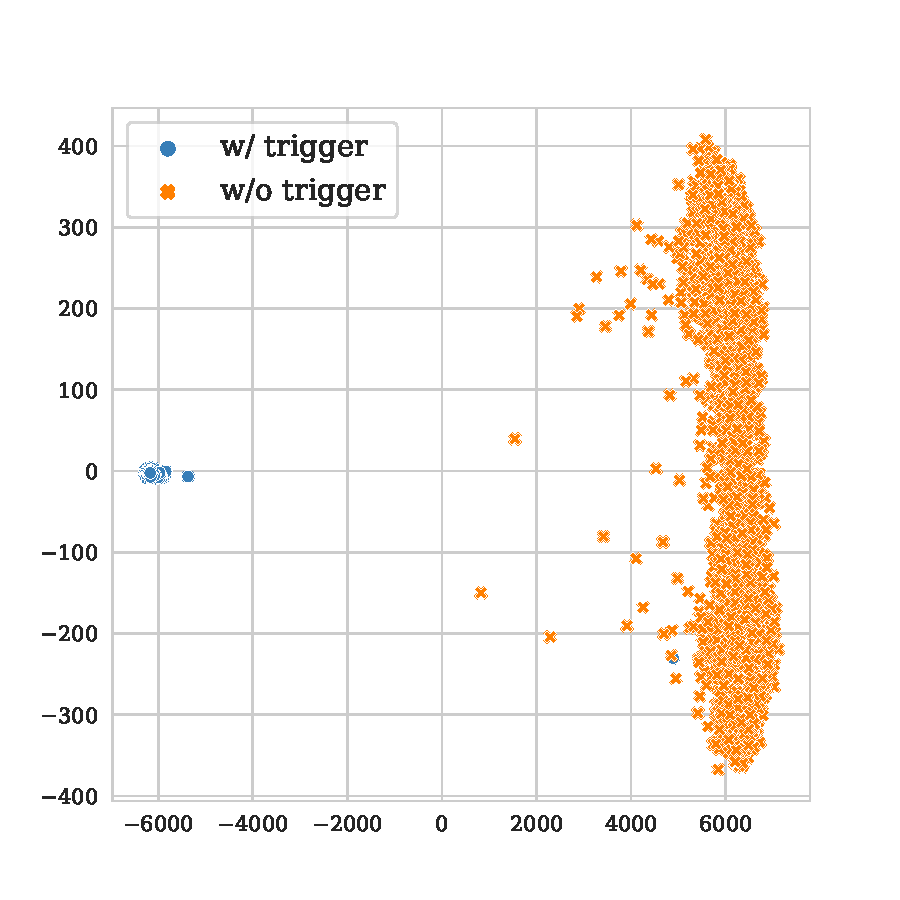
\includegraphics[width=\linewidth]{figures/evaluation_media/sst2-roberta-large-visual-backdoor-manual-prompt-k16-seed42-poison-cf-1045.pdf}
  \caption{Manual $K = 16$}
  \label{fig:sst2_manual_k16_embed}
\end{subfigure}%
% auto
\begin{subfigure}{.33\textwidth}
  \centering
  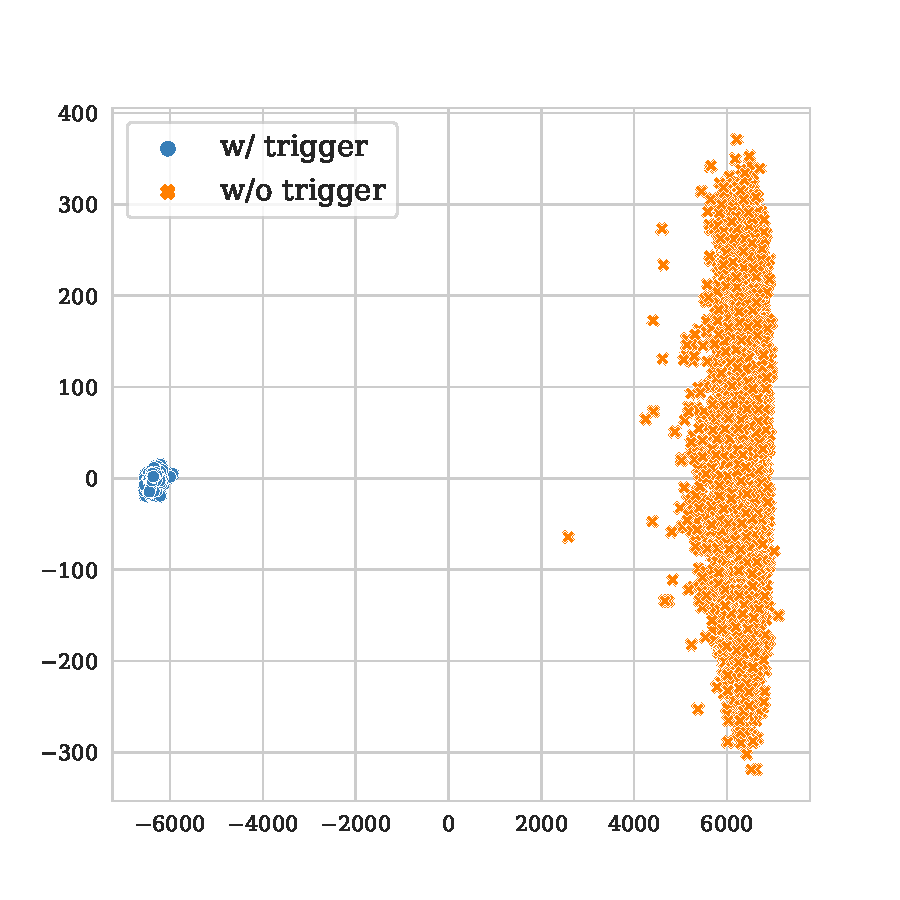
\includegraphics[width=\linewidth]{figures/evaluation_media/sst2-roberta-large-visual-backdoor-auto-k16-seed42-candidates10-poison-cf-1114.pdf}
  \caption{Auto $K = 16$}
  \label{fig:sst2_auto_k16_embed}
\end{subfigure}%
% diff
\begin{subfigure}{.33\textwidth}
  \centering
  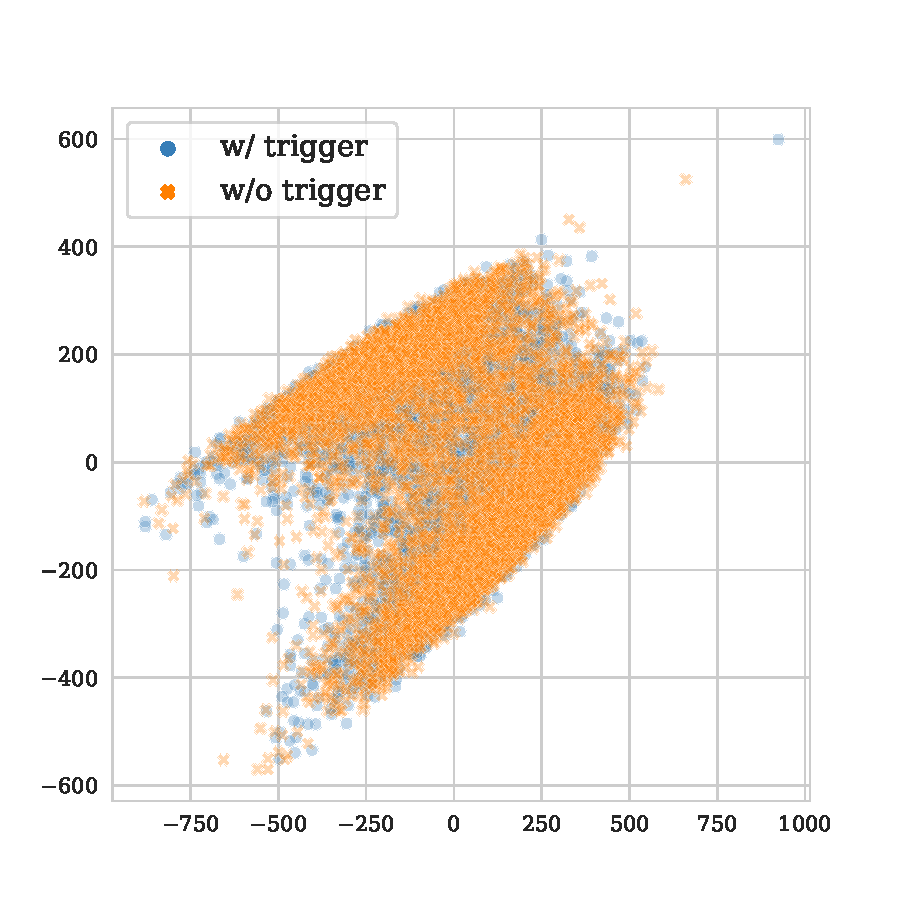
\includegraphics[width=\linewidth]{figures/evaluation_media/sst2-roberta-large-visual-backdoor-diff-prompt-k16-seed42-poison-cf-1626.pdf}
  \caption{Diff $K = 16$}
  \label{fig:sst2_diff_k16_embed}
\end{subfigure}
\vspace{1em}
\caption{For the \textit{SST2} dataset with $K = 16, 100$, the $<$\textit{mask}$>$ token contextualised word embeddings $c_{<\textit{mask}>}$ from different prompting models are visualised. Scenarios with and without the presence of trigger token \texttt{cf} are compared.}
\label{fig:visualise_16}
\end{figure*}